\section{\scalenetcdf ファイルとは?} \label{sec:netcdf}
本節では、{\scalelib}が直接読み書きする{\scalenetcdf}ファイルについて説明する。
\scalelib では、データファイルの形式として{\netcdf}(network Common Data Format)を採用している。
\Netcdf は Unidata (\url{http://www.unidata.ucar.edu}) が開発を行っているソフトウェアであり、自己記述的で計算機に依存しないデータ形式のファイルを生成することを可能にする。
例えば、前者についてはファイル中に軸変数と一緒に変数を記述できる長所がある。
また、後者については、どのエンディアンが使用されるかを気にせずにデータを扱える長所がある。
\scalelib では、上記の利点に基づいてある規約(\scalenetcdf convention )を定めている。
この規約は、CF convection (\url{http://cfconventions.org})におおよそ従っている。

\subsection{グローバル属性}
\scalenetcdf ファイルには、ファイルに含まれるデータの情報(空間分割に関する情報等)がグローバル属性(global attribute)として格納されている(表\ref{table:netcdf_global_attrs})。

\begin{table}
  \begin{center}
    \caption{\scalenetcdf ファイルのグローバル属性}
    \label{table:netcdf_global_attrs}
    \begin{tabularx}{150mm}{p{50mm}XX} \hline
      名前        & 説明                 & 備考 \\ \hline \hline
      title       & データの簡潔な説明   & \namelist{PARAM_FILE_HISTORY}の\nmitem{FILE_History_TITLE}の値  \\
      source      & ソフトウエア名 & ヒストリファイルに対しては\namelist{PARAM_FILE_HISTORY}の\nmitem{FILE_History_SOURCE}の値。他のファイルに対しては\namelist{PARAM_IO}の\nmitem{H_SOURCE}の値\\
      institution & データ作成者               & ヒストリファイルに対しては\namelist{PARAM_FILE_HISTORY}の\nmitem{FILE_History_INSTITUTION}の値。他のファイルに対しては\namelist{PARAM_IO}の\nmitem{H_INSTITUTE}の値\\
      rankid      & MPI プロセスのランク番号      & モデルの\verb|PRC_myrank| \\
      Conventions & CF 規約のバージョン       & ``CF-1.6'' for version 5.3 \\
      grid\_name  & 格子の種類                   & \scalerm では``cartesC''  \\
      scale\_cartesC\_prc\_rank\_[xy]           & 二次元分割のマッピング番号      & モデルにおいて変数\verb|PRC_2Drank(PRC_myrank, i)|に等しい(x: i=1, y: i=2)\\
      scale\_cartesC\_prc\_num\_[xy]            & 二次元分割数            & モデルでは、~\nmitem{PRC_NUM_X}, \nmitem{PRC_NUM_Y} \\
      scale\_cartesC\_prc\_periodic\_[zxy]      & 境界条件が周期的か? & \verb|.false.|or\verb|.true.|\ モデルでは\nmitem{PRC_PERIODIC_X}, \nmitem{PRC_PERIODIC_Y} に対応 \\
      scale\_atmos\_grid\_cartesC\textbackslash \ ~~\_index\_[ij]maxg  & 領域全体の格子点数               & モデルにおいて、 ~\nmitem{IMAX}$\times$\nmitem{PRC_NUM_X}, \nmitem{JMAX}$\times$\nmitem{PRC_NUM_Y}  \\
      scale\_atmos\_grid\_cartesC\textbackslash \ ~~\_index\_kmax      & 大気モデルの鉛直層数 & モデルでは~\nmitem{KMAX} \\
      scale\_ocean\_grid\_cartesC\textbackslash \ ~~\_index\_kmax      & 海洋モデルの鉛直層数       & モデルでは~\nmitem{OKMAX} \\
      scale\_land\_grid\_cartesC\textbackslash \ ~~\_index\_kmax       & 陸モデルの鉛直層数        & モデルでは~\nmitem{LKMAX}  \\
      scale\_urban\_grid\_cartesC\textbackslash \ ~~\_index\_kmax      & 都市モデルの鉛直層数       & モデルでは ~\nmitem{UKMAX} \\
      scale\_atmos\_grid\_cartesC\textbackslash \ ~~\_index\_[kij]halo & ハロの格子数                                   & モデルでは~\nmitem{KHALO}, \nmitem{IHALO}, \nmitem{JHALO} \\
      Calendar    & 暦の種類                            & モデルでは~\nmitem{PARAM_CALENDAR} \\
      time\_units & 時間の単位 & \\
      time\_start & 開始時刻   & \\ \hline
      \multicolumn{3}{l}{\nmitem{History_TITLE, History_SOURCE, History_INSTITUTION}は第\ref{sec:output}節を参照。} \\
      \multicolumn{3}{l}{\nmitem{PRC_NUM_X, PRC_NUM_Y, PRC_PERIODIC_X, PRC_PERIODIC_Y}、\nmitem{KMAX, IMAX, JMAX}は第\ref{sec:domain}節を参照。}  \\
      \multicolumn{3}{l}{\nmitem{PARAM_CALENDAR}は第\ref{subsec:calendar}節を参照。} \\ \hline
    \end{tabularx}
  \end{center}
\end{table}

\noindent \nmitem{PRC_NUM_X, PRC_NUM_Y}については、第\ref{sec:domain}節を参照されたい。


\subsection{ハロ領域データ}
ファイルにハロ領域データが含まれるかは、ファイルの種類や設定によって依存する。
ただし、ここで定義するハロ領域とは計算領域全体に対するハロであり、
各々の局所領域に対するハロを意味しないことに注意されたい。

初期値(またはリスタート)データおよび境界値データについては、側面境界条件が周期境界でない場合 (\namelist{PARAM_PRC_CARTESC}において\nmitem{PRC_PERIODIC_X}と\nmitem{PRC_PERIODIC_Y}を\verb|.false.|とした場合)、もしくは単一ファイルの入出力の場合(\namelist{PARAM_IO}の\nmitem{IO_AGGREGATE}を\verb|.true.|とした場合)にはハロ領域データが含まれる。
それ以外の場合、ハロ領域データは含まれない。

一方で、ヒストリデータについては、側面境界条件が周期的でなく、
かつ\namelist{PARAM_HIST}の\nmitem{HIST_BND}を\verb|.true.|とした場合にはハロ領域データが含まる。
それ以外の場合、ハロ領域データは含まれない。
詳細は第\ref{sec:output}節を参照されたい。


\subsection{軸変数}
\scalenetcdf ファイルには、軸に関するデータが格納されている。
全ての軸変数は「long\_name」と「units」の属性を持ち、
これらはそれぞれ変数の説明や単位を記述する。
また、x, y, xh, yh には、全領域データ格子数(size\_global)、
ファイルに含まれるデータの全格子中での開始格子点位置(start\_global)、
全領域データにおける先頭および末尾におけるハロ領域の格子数(halo\_global)、
ファイルに含まれるデータのハロ領域の格子数(halo\_local) に関する属性が付加されている。

表\ref{table:netcdf_axes}に、軸データのリストを示す。
座標変数は自身の次元を持ち、その変数名は次元名と同じである。
小文字の名前の変数はファイルの中で主に用いられ、
一方で大文字の名前の変数は計算で用いられる軸を表す。
図\ref{fig:netcdfhorizontalcoordinate}と図\ref{fig:netcdfverticalcoordinate}はそれぞれ、座標変数の水平位置や鉛直位置を示している。
同時に、表\ref{table:netcdf_axes}も参照されたい。

格子の面積データや体積データもそれぞれ、「cell\_area**」と「cell\_volume**」としてファイルに格納されている。
各変数の「cell\_measures」属性には、対応する面積や体積データを指定する。

地図投影データは無次元変数として格納されおり、これらの名前は変数の属性「grid\_mapping」で指定する。

スタッガード格子の位置関係に関する情報は、SGRID 規約(\url{https://github.com/sgrid/sgrid})に基づいて、
属性や無次元変数として格納している。
その無次元変数の名前は、各変数の「grid」属性で指定される。

ファイルには、地表面高度データ「topo」や陸に対するマスクのデータ「lsmask」も含まれる。


\begin{longtable}{l|l}
  \caption{\scalenetcdf に含まれる軸データ.}
  \label{table:netcdf_axes} \\ \hline
  \endfirsthead
  \multicolumn{2}{l}{\small\it 前ページからの続き..} \\ \hline
%  & name & description \\ \hline \hline
  \endhead
  \hline
  \endfoot
  \multicolumn{2}{l}{座標変数}\\ \hline
名前 & 説明 \\ \hline \hline
\multicolumn{2}{c}{水平軸 \& 時間軸: 共通}\\ \hline
x        & ファイルに含まれるデータの x 方向の full level の位置 \\
x\_bnds  & ファイルに含まれるデータの x 方向の full level のセル境界 \\
xh       & ファイルに含まれるデータの x 方向の half level の位置 \\
xh\_bnds & ファイルに含まれるデータの x 方向の half level のセル境界 \\
y        & ファイルに含まれるデータの y 方向の full level の位置 \\
y\_bnds  & ファイルに含まれるデータの y 方向の full level のセル境界 \\
yh       & ファイルに含まれるデータの y 方向の half level の位置 \\
yh\_bnds & ファイルに含まれるデータの y 方向の half level のセル境界 \\
time       & 時刻の情報 \\ \hline
time\_bnds & 時刻の境界情報 \\ \hline
CX  & 局所領域に対する x 方向の full level の格子位置 (ハロ格子を含む) \\
FX  & 局所領域に対する x 方向の half level の格子位置 (ハロ格子を含む) \\
CDX & x 方向の  full level の格子間隔 (ハロ格子を含む)  \\
FDX & x 方向の  half level の格子間隔 (ハロ格子を含む) \\
CY  & 局所領域に対する y 方向の full level の格子位置 (ハロ格子を含む) \\
FY  & 局所領域に対する y 方向の half level の格子位置 (ハロ格子を含む)\\
CDY & y 方向の  full level の格子間隔 (ハロ格子を含む) \\
FDY & y 方向の  half level の格子間隔 (ハロ格子を含む) \\
CXG & 全領域に対する x 方向の full level の格子位置 (ハロ格子を含む) \\
FXG & 全領域に対する x 方向の half level の格子位置 (ハロ格子を含む) \\
CYG & 全領域に対する y 方向の full level の格子位置 (ハロ格子を含む) \\
FYG & 全領域に対する y 方向の half level の格子位置 (ハロ格子を含む) \\ \hline
\multicolumn{2}{c}{鉛直軸 : 大気}\\ \hline
z         & ファイルに含まれる大気データの z 方向の full level の位置 \\
z\_bnds   & ファイルに含まれる大気データの z 方向の full level のセル境界 \\
zh        & ファイルに含まれる大気データの z 方向の half level の位置 \\
zh\_bnds  & ファイルに含まれる大気データの z 方向の half level のセル境界 \\
CZ  & 大気モデルの z 方向の full level の格子位置 (ハロ格子を含む) \\
FZ  & 大気モデルの z 方向の half level の格子位置 (ハロ格子を含む) \\
CDZ & 大気モデルの z 方向の full level の格子間隔 (ハロ格子を含む) \\
FDZ & 大気モデルの z 方向の half level の格子間隔 (ハロ格子を含む) \\ \hline
\multicolumn{2}{c}{鉛直軸 : 海洋}\\ \hline
oz        & ファイルに含まれる海洋データの z 方向の full level の位置 \\
oz\_bnds  & ファイルに含まれる海洋データの z 方向の full level のセル境界 \\
ozh       & ファイルに含まれる海洋データの z 方向の half level の位置 \\
ozh\_bnds & ファイルに含まれる海洋データの z 方向の half level のセル境界 \\
OCZ  & 海洋モデルの z 方向の full level の格子位置 \\
OFZ  & 海洋モデルの z 方向の half level の格子位置 \\
OCDZ & 海洋モデルの z 方向の full level の格子間隔 \\  \hline
\multicolumn{2}{c}{鉛直軸 : 陸面}\\ \hline
lz        & ファイルに含まれる陸面データの z 方向の full level の位置 \\
lz\_bnds  & ファイルに含まれる陸面データの z 方向の full level のセル境界 \\
lzh       & ファイルに含まれる陸面データの z 方向の half level の位置 \\
lzh\_bnds & ファイルに含まれる陸面データの z 方向の half level のセル境界 \\
LCZ  & 陸面モデルの z 方向の full level の格子位置 \\
LFZ  & 陸面モデルの z 方向の half level の格子位置 \\
LCDZ & 陸面モデルの z 方向の full level の格子間隔 \\  \hline
\multicolumn{2}{c}{鉛直軸: 都市キャノピー}\\ \hline
uz        & ファイルに含まれる都市データの z 方向の full level の位置 \\
uz\_bnds  & ファイルに含まれる都市データの z 方向の full level のセル境界 \\
uzh       & ファイルに含まれる都市データの z 方向の half level の位置 \\
uzh\_bnds & ファイルに含まれる陸面データの z 方向の half level のセル境界 \\
UCZ  & 都市モデルの z 方向の full level の格子位置 \\
UFZ  & 都市モデルの z 方向の half level の格子位置 \\
UCDZ & 都市モデルの z 方向の full level の格子間隔 \\ \hline
 \hline
  \multicolumn{2}{l}{他の軸変数(1D)}\\ \hline
名前  & 説明 \\ \hline \hline
CBFZ  & CZ でのバッファ係数 \\
FBFZ  & FZ でのバッファ係数 \\
CBFX  & 局所領域に対する CX でのバッファ係数 \\
FBFX  & 局所領域に対する FX でのバッファ係数 \\
CBFY  & 局所領域に対する CY でのバッファ係数 \\
FBFY  & 局所領域に対する FY でのバッファ係数 \\
CBFXG & 全領域に対する CXG でのバッファ係数 \\
FBFXG & 全領域に対する FXG でのバッファ係数 \\
CBFYG & 全領域に対する CYG でのバッファ係数 \\
FBFYG & 全領域に対する FYG でのバッファ係数 \\
\hline
\multicolumn{2}{l}{他の軸変数 (2D)}\\ \hline
名前 & 説明 \\ \hline \hline
lon     & (y, x) での経度 \\
lon\_uy & (y, xh) での経度 \\
lon\_xv & (yh, x) での経度 \\
lon\_uv & (yh, xh) での経度 \\
lat     & (y, x) での緯度  \\
lat\_uy & (y, xh) での緯度 \\
lat\_xv & (yh, x) での緯度 \\
lat\_uv & (yh, xh) での緯度 \\
\hline
\multicolumn{2}{l}{他の軸変数 (3D)}\\ \hline
名前 & 説明 \\ \hline \hline
height      & ヒストリファイル中の(z,y,x) orリスタート/初期値ファイル中の(y,x,z)での高度\\
height\_xyw & ヒストリファイル中の(zh,y,x) orリスタート/初期値ファイル中の(y,x,zh)での高度\\
height\_xvz & ヒストリファイル中の(z,yh,x) orリスタート/初期値ファイル中の(yh,x,z)での高度\\
height\_uyz & ヒストリファイル中の(z,y,xh) orリスタート/初期値ファイル中の(y,xh,z)での高度\\
height\_xvw & ヒストリファイル中の(z,yh,x) orリスタート/初期値ファイル中の(yh,x,z)での高度\\
height\_uyw & ヒストリファイル中の(zh,y,xh) orリスタート/初期値ファイル中の(y,xh,zh)での高度\\
height\_uvz & ヒストリファイル中の(z,yh,xh) orリスタート/初期値ファイル中の(yh,xh,z)での高度\\
height\_uvw & ヒストリファイル中の(zh,yh,xh) orリスタート/初期値ファイル中の(yh,xh,zh)での高度\\
\end{longtable}

\begin{figure}[tbh]
\begin{center}
  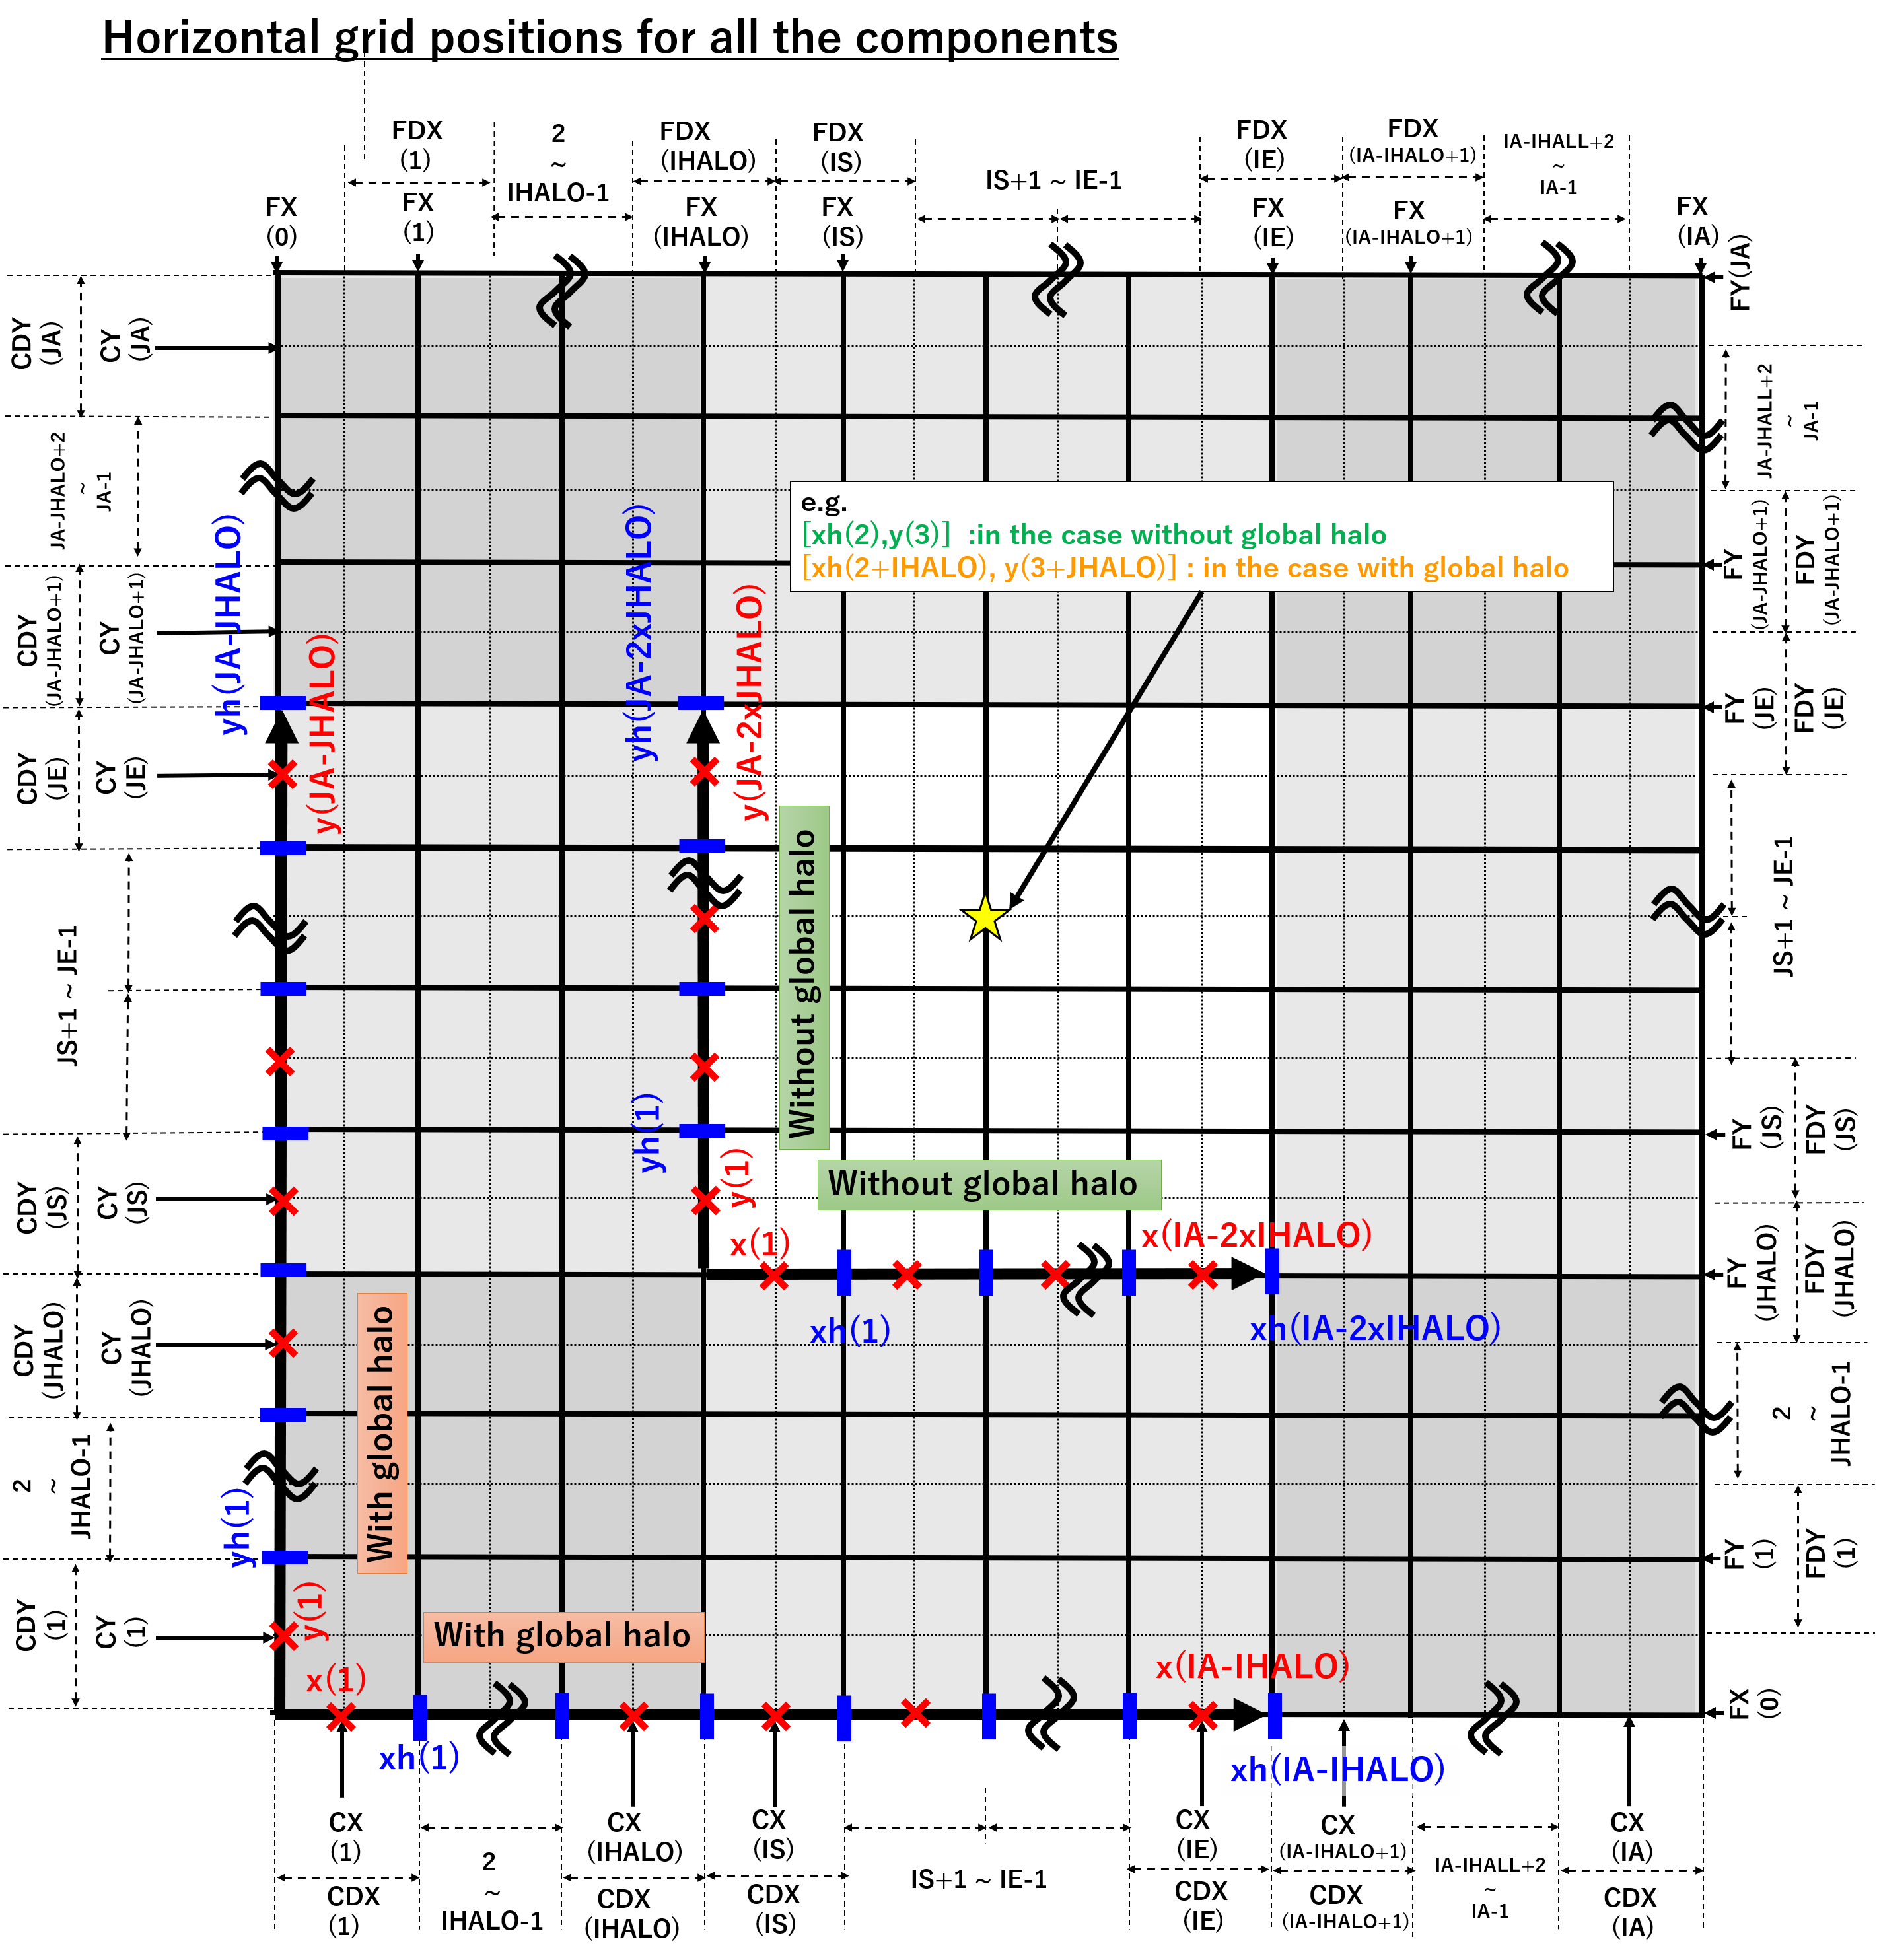
\includegraphics[width=1.0\hsize]{./../../figure/horizontal-coordinate-final2.png}\\
  \caption{{\scalenetcdf}ファイルにおける水平座標}
  \label{fig:netcdfhorizontalcoordinate}
\end{center}
\end{figure}
\begin{figure}[tbh]
\begin{center}
  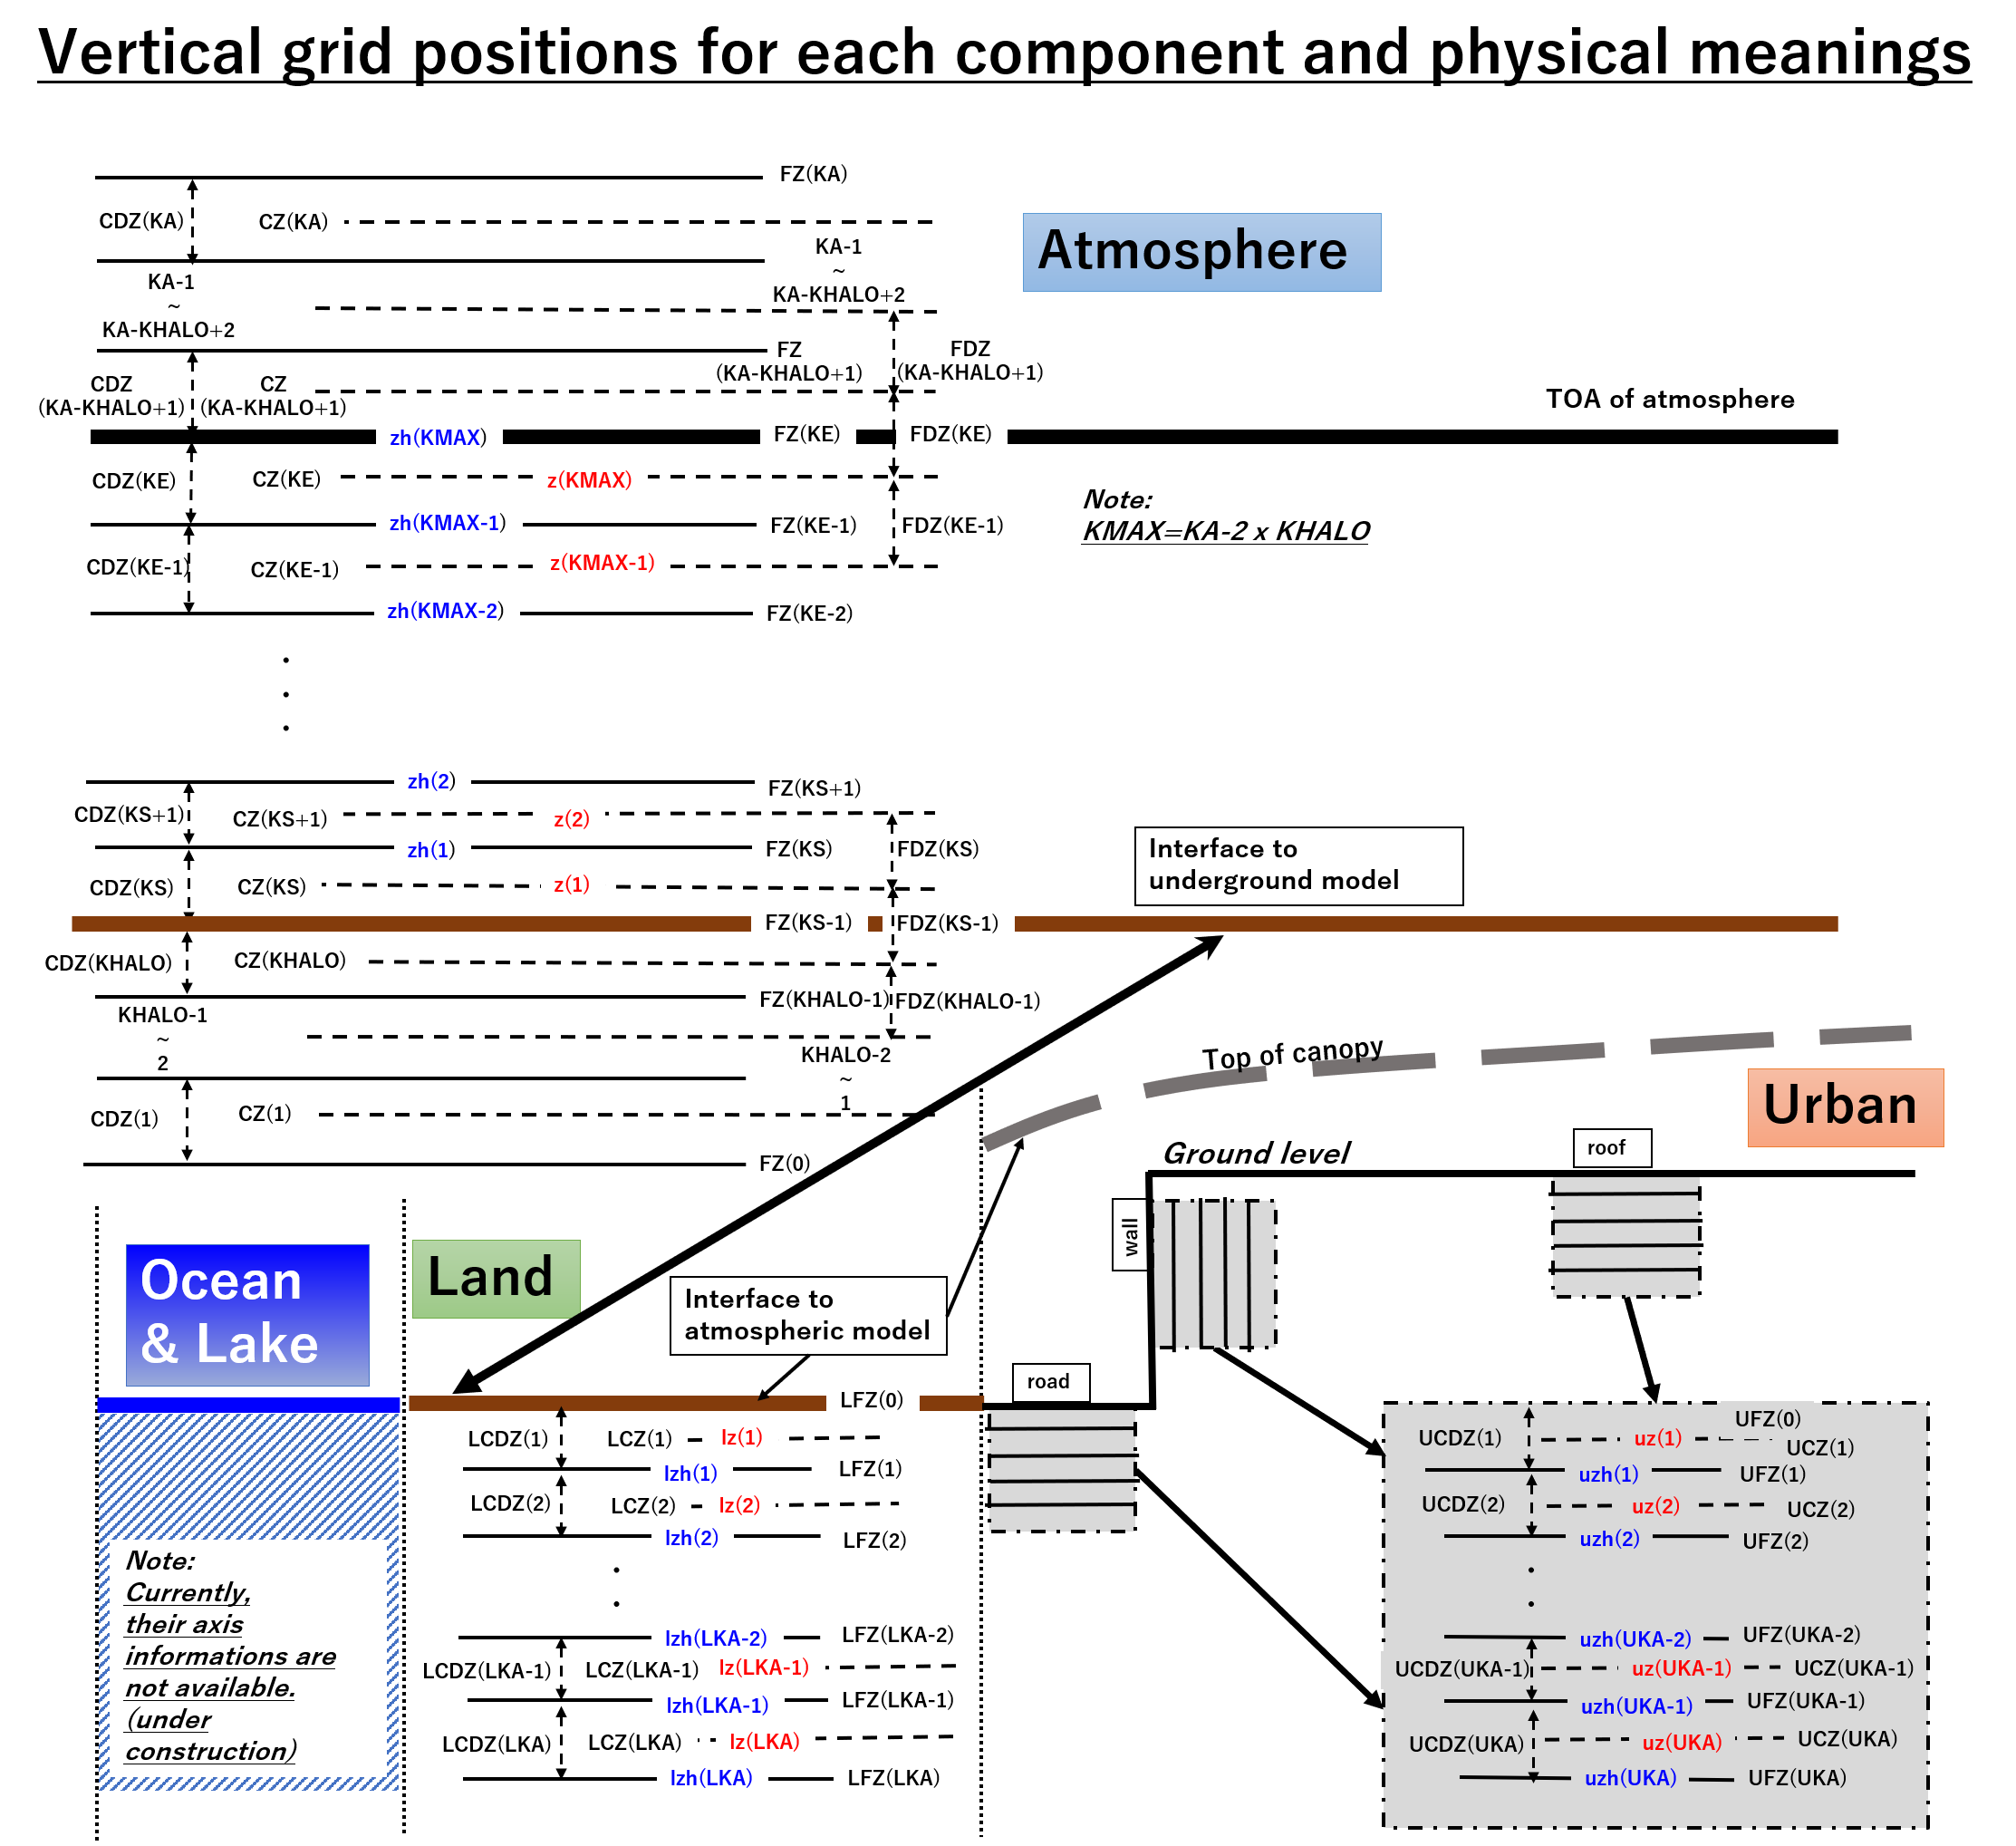
\includegraphics[width=1.0\hsize]{./../../figure/vertical_coordinate_final2.png}\\
  \caption{{\scalenetcdf}ファイルにおける鉛直座標}
  \label{fig:netcdfverticalcoordinate}
\end{center}
\end{figure}

\subsection{データ変数}
データ変数は、long\_name, units に加えて、未定義値を表す \_FillValue や欠損値を表す missing\_value を属性として持っている。

初期値(リスタート)データファイル、境界値データのデータ構造はモデル内の配列構造と同じで、z, x, y の順番である。
一方、ヒストリデータファイルは、x, y, z の順番である。

\subsection{単一ファイルの入出力} \label{subsec:single_io}
デフォルトでは、全てのデータファイルは各プロセスごとに出力される。
つまり、ファイルI/O は各プロセスで独立である。
pnetCDF を使用するように \scalerm をコンパルした場合(環境変数を SCALE\_ENABLE\_PNETCDF=T と設定してコンパルした場合)は、全プロセスからのデータを単一ファイルにまとめることができる(第\ref{subsec:environment}節を参照)。
これを行うには、 \namelist{PARAM_FILE}の\nmitem{FILE_AGGREGATE}を\verb|.true.|に設定する必要がある。
あるいは、ヒストリ、地形、土地利用区分ファイルといった個々のファイルの種類に対して、
単一ファイルの入出力を切り替えることもできる。
ヒストリファイルについては、 \namelist{PARAM_FILE_HISTORY}の\nmitem{FILE_HISTORY_AGGREGATE}を\verb|.true.|にすれば良い。
初期値/リスタートファイルについては、\namelist{PARAM_RESTART}の\nmitem{RESTART_(IN|OUT)_AGGREGATE}、または\namelist{PARAM_(MODELNAME)_VARS}の
\nmitem{(MODELNAME)_RESTART_(IN|OUT)_AGGREGATE}を\verb|.true.|にすれば良い。
ただし、\verb|(MODELNAME)|には「ATMOS」、「OCEAN」、「LAND」、「URBAN」が入る。
地形ファイルや土地利用区分ファイルについてはそれぞれ、\namelist{PARAM_TOPOGRAPHY}の\\\nmitem{TOPOGRAPHY_(IN|OUT)_AGGREGATE}や\namelist{PARAM_LANDUSE}の\nmitem{LANDUSE_(IN|OUT)_AGGREGATE}を\verb|.true.|にすれば良い。

\subsection{\Netcdf 3 に伴う制限}
{\netcdf} version 3 と共に\scale をコンパイルした場合は、次の制限が存在する。
\begin{itemize}
\item 異なる時間間隔の変数は、同じファイルに出力できない。
\item データ圧縮が使用できない。
\item {\netcdf}4 形式のファイルは読み込めない。
\end{itemize}
異なる時間間隔で変数を出力したい場合は、それらを異なるファイルに出力するために\namelist{HISTORY_ITEM}の\nmitem{BASENAME}を設定されたい。

pnetCDF は \netcdf 3 のファイル形式に基づくので、
単一ファイルの入出力機能を用いる場合は複数の時間間隔や圧縮が制限されることに注意が必要である。

\begin{table}
  \caption{{\netcdf}の各バージョンの機能性}
  \begin{tabular}{llllll} \hline
    & \shortstack{複数の\\時間間隔} & 圧縮 & \shortstack{\netcdf 3 ファイルの\\読み込み} & \shortstack{\netcdf 4 ファイルの\\読み込み} & \shortstack{単一ファイルの\\読み込み}\\ \hline
    \netcdf 3 & NG & NG & OK & NG & NG$^{*}$ \\
    \netcdf 4 & OK & OK & OK & OK & NG$^{*}$ \\
    pnetCDF   & NG & NG & NG$^{*}$ & NG & OK \\\hline
  \end{tabular}
  \\
  (*) 全プロセス数が 1 であれば読み込み可能
\end{table}
